\documentclass[11pt,a4paper]{jsarticle}
\usepackage{amsmath,amssymb}
\usepackage{amsthm}
\usepackage{ascmac}
\usepackage{bm}
\usepackage[dvipdfmx]{graphicx}	% required for `\includegraphics' (yatex added)
\usepackage{setspace}           % required for `\doublespace'
\usepackage{tikz}
\usepackage{tikz-cd}
\usetikzlibrary{angles, positioning, shapes, arrows.meta, decorations.pathmorphing}
%\usetikzlibrary{intersections, calc, arrows, positioning, arrows.meta}
\usepackage{tcolorbox}  % 定理環境の装飾
\tcbuselibrary{skins, breakable, theorems}
\usepackage{xcolor}
\usepackage{natbib}
\usepackage{pxrubrica}
\usepackage[margin=30truemm, left=40truemm, right=40truemm]{geometry}
\usepackage{thmbox}     % required for theorem environment with side bar
%
\setlength{\parskip}{3mm} %段落間にスペースを入れる


% \pagestyle{myheadings}
% \markright{\footnotesize \sf 2022秋期「哲学者のための数学」授業資料(大塚淳) \ \ 配布禁止}


\theoremstyle{definition}
\newtheorem[S]{exercise}{練習問題}[section]
\newtheorem[S]{example}{事例}[section]
\newtheorem[S]{fact}{事実}[section]
\newtheorem[S]{attn}{注意}[section]
\newtheorem[S]{develop}{発展}[section]
\renewcommand{\theattn}{}

\newtcbtheorem[auto counter, number within=section]{rei}{事例}{
    breakable,
    coltitle=black,
    fonttitle=\bfseries,
    enhanced, colback=white, frame hidden, borderline west = {0.5pt}{5pt}{black},
%    number freestyle={\noexpand\thesection.\noexpand\arabic{\tcbcounter}}
}{rei}

\newtcbtheorem[auto counter, number within=section]{prop}{命題}{
    breakable,
    coltitle=black,
    fonttitle=\bfseries,
    enhanced, colback=white, frame hidden, borderline west = {0.5pt}{5pt}{black},
%    number freestyle={\noexpand\thesection.\noexpand\arabic{\tcbcounter}}
}{prop}

\newtcbtheorem[number within=section]{renshu}{練習問題}{
    breakable,
    coltitle=black,
    fonttitle=\bfseries,
    enhanced, colback=white, frame hidden, borderline west = {0.5pt}{5pt}{black}
}{renshu}


\newtcbtheorem[number within=section]{hatten}{発展}{
    breakable,
    coltitle=black,
    fonttitle=\bfseries,
    enhanced, colback=white, frame hidden, borderline west = {0.5pt}{5pt}{black}
}{renshu}


\newtcbtheorem[number within=section]{dfn}{定義}{
    fonttitle=\bfseries,
    enhanced, colback=white
}{dfn}


% Bold face capital letters:
\newcommand{\bfzero}{\boldsymbol{0}}
\newcommand{\bfone}{\boldsymbol{1}}
\newcommand{\bfA}{\boldsymbol{A}}
\newcommand{\bfB}{\boldsymbol{B}}
\newcommand{\bfC}{\boldsymbol{C}}
\newcommand{\bfD}{\boldsymbol{D}}
\newcommand{\bfE}{\boldsymbol{E}}
\newcommand{\bfF}{\boldsymbol{F}}
\newcommand{\bfG}{\boldsymbol{G}}
\newcommand{\bfH}{\boldsymbol{H}}
\newcommand{\bfI}{\boldsymbol{I}}
\newcommand{\bfJ}{\boldsymbol{J}}
\newcommand{\bfK}{\boldsymbol{K}}
\newcommand{\bfL}{\boldsymbol{L}}
\newcommand{\bfM}{\boldsymbol{M}}
\newcommand{\bfN}{\boldsymbol{N}}
\newcommand{\bfO}{\boldsymbol{O}}
\newcommand{\bfP}{\boldsymbol{P}}
\newcommand{\bfQ}{\boldsymbol{Q}}
\newcommand{\bfR}{\boldsymbol{R}}
\newcommand{\bfS}{\boldsymbol{S}}
\newcommand{\bfT}{\boldsymbol{T}}
\newcommand{\bfU}{\boldsymbol{U}}
\newcommand{\bfV}{\boldsymbol{V}}
\newcommand{\bfW}{\boldsymbol{W}}
\newcommand{\bfX}{\boldsymbol{X}}
\newcommand{\bfY}{\boldsymbol{Y}}
\newcommand{\bfZ}{\boldsymbol{Z}}

\newcommand{\bfa}{\boldsymbol{a}}
\newcommand{\bfb}{\boldsymbol{b}}
\newcommand{\bfc}{\boldsymbol{c}}
\newcommand{\bfd}{\boldsymbol{d}}
\newcommand{\bfe}{\boldsymbol{e}}
\newcommand{\bff}{\boldsymbol{f}}
\newcommand{\bfk}{\boldsymbol{k}}
\newcommand{\bfm}{\boldsymbol{m}}
\newcommand{\bfn}{\boldsymbol{n}}
\newcommand{\bfo}{\boldsymbol{o}}
\newcommand{\bfp}{\boldsymbol{p}}
\newcommand{\bfq}{\boldsymbol{q}}
\newcommand{\bfr}{\boldsymbol{r}}
\newcommand{\bfs}{\boldsymbol{s}}
\newcommand{\bft}{\boldsymbol{t}}
\newcommand{\bfu}{\boldsymbol{u}}
\newcommand{\bfv}{\boldsymbol{v}}
\newcommand{\bfw}{\boldsymbol{w}}
\newcommand{\bfx}{\boldsymbol{x}}
\newcommand{\bfy}{\boldsymbol{y}}
\newcommand{\bfz}{\boldsymbol{z}}



% BB (???) capital letters:
\newcommand{\bbA}{\mathbb{A}}
\newcommand{\bbB}{\mathbb{B}}
\newcommand{\bbC}{\mathbb{C}}
\newcommand{\bbD}{\mathbb{D}}
\newcommand{\bbE}{\mathbb{E}}
\newcommand{\bbF}{\mathbb{F}}
\newcommand{\bbG}{\mathbb{G}}
\newcommand{\bbI}{\mathbb{I}}
\newcommand{\bbN}{\mathbb{N}}
\newcommand{\bbP}{\mathbb{P}}
\newcommand{\bbQ}{\mathbb{Q}}
\newcommand{\bbR}{\mathbb{R}}
\newcommand{\bbU}{\mathbb{U}}
\newcommand{\bbV}{\mathbb{V}}
\newcommand{\bbX}{\mathbb{X}}
\newcommand{\bbY}{\mathbb{Y}}
\newcommand{\bbZ}{\mathbb{Z}}
\newcommand{\bbone}{{\ifmmode\mathrm{1\!l}\else\mbox{\(\mathrm{1\!l}\)}\fi}}


% Caligraphic math capital letters:
\newcommand{\mcalA}{\mathcal{A}}
\newcommand{\mcalB}{\mathcal{B}}
\newcommand{\mcalC}{\mathcal{C}}
\newcommand{\mcalD}{\mathcal{D}}
\newcommand{\mcalE}{\mathcal{E}}
\newcommand{\mcalF}{\mathcal{F}}
\newcommand{\mcalG}{\mathcal{G}}
\newcommand{\mcalH}{\mathcal{H}}
\newcommand{\mcalI}{\mathcal{I}}
\newcommand{\mcalJ}{\mathcal{J}}
\newcommand{\mcalK}{\mathcal{K}}
\newcommand{\mcalL}{\mathcal{L}}
\newcommand{\mcalM}{\mathcal{M}}
\newcommand{\mcalN}{\mathcal{N}}
\newcommand{\mcalO}{\mathcal{O}}
\newcommand{\mcalP}{\mathcal{P}}
\newcommand{\mcalQ}{\mathcal{Q}}
\newcommand{\mcalS}{\mathcal{S}}
\newcommand{\mcalT}{\mathcal{T}}
\newcommand{\mcalU}{\mathcal{U}}
\newcommand{\mcalV}{\mathcal{V}}
\newcommand{\mcalX}{\mathcal{X}}
\newcommand{\mcalY}{\mathcal{Y}}
\newcommand{\mcalZ}{\mathcal{Z}}

% Graph nodes notations:
\newcommand{\PA}{\mathit{PA}}
\newcommand{\bfPA}{\mathbf{PA}}
\newcommand{\CH}{\mathit{CH}}
\newcommand{\bfCH}{\mathbf{CH}}
\newcommand{\DS}{\mathit{DS}}
\newcommand{\bfDS}{\mathbf{DS}}
\newcommand{\ND}{\mathit{ND}}
\newcommand{\bfND}{\mathbf{ND}}
\newcommand{\AN}{\mathit{an}}
\newcommand{\bfAN}{\mathbf{an}}
\newcommand{\pa}{\mathit{pa}}
\newcommand{\bfpa}{\mathbf{pa}}
\newcommand{\ch}{\mathit{ch}}
\newcommand{\bfch}{\mathbf{ch}}
\newcommand{\ds}{\mathit{ds}}
\newcommand{\bfds}{\mathbf{ds}}
\newcommand{\nd}{\mathit{nd}}
\newcommand{\bfnd}{\mathbf{nd}}
\newcommand{\an}{\mathit{an}}
\newcommand{\bfan}{\mathbf{an}}



\DeclareMathOperator*{\argmax}{arg\,max}
\DeclareMathOperator*{\argmin}{arg\,min}
\DeclareMathOperator*{\argsup}{arg\,sup}
\DeclareMathOperator*{\arginf}{arg\,inf}
\DeclareMathOperator{\erfc}{erfc}
\DeclareMathOperator{\diag}{diag}
\DeclareMathOperator{\cum}{cum}
\DeclareMathOperator{\sgn}{sgn}
\DeclareMathOperator{\tr}{tr}
\DeclareMathOperator{\spn}{span}
\DeclareMathOperator{\adj}{adj}
\DeclareMathOperator{\E}{\mathbb{E}}
\DeclareMathOperator{\var}{Var}
\DeclareMathOperator{\cov}{Cov}
\DeclareMathOperator{\corr}{corr}
\DeclareMathOperator{\sech}{sech}
\DeclareMathOperator{\sinc}{sinc}
\DeclareMathOperator*{\lms}{l.i.m.\,}
\newcommand{\varop}[1]{\var\left[{#1}\right]}
\newcommand{\covop}[2]{\cov\left({#1},{#2}\right)}
\newcommand{\T}{^\textrm{T}}
\newcommand\indep{\protect\mathpalette{\protect\independenT}{\perp}}
\def\independenT#1#2{\mathrel{\rlap{$#1#2$}\mkern2mu{#1#2}}}

\newcommand{\bfalpha}{\boldsymbol{\alpha}}
\newcommand{\bfbeta} {\boldsymbol{\beta}}
\newcommand{\bfgamma}{\boldsymbol{\gamma}}
\newcommand{\bfeta}  {\boldsymbol{\eta}}
\newcommand{\bftheta}{\boldsymbol{\theta}}
\newcommand{\bflambda}   {\boldsymbol{\lambda}}
\newcommand{\bfmu}   {\boldsymbol{\mu}}
\newcommand{\bfnu}   {\boldsymbol{\nu}}
\newcommand{\bfxi}   {\boldsymbol{\xi}}
\newcommand{\bfpsi}  {\boldsymbol{\psi}}
\newcommand{\bfphi}   {\boldsymbol{\phi}}
\newcommand{\bfrho}   {\boldsymbol{\rho}}
\newcommand{\bfvarepsilon}{\boldsymbol{\varepsilon}}
%\newcommand{\qed}{{qed}}
%\newcommand{\eqalignno}[1]{\begin{array}{ccccccc}#1\end{array}}

\newcommand{\bfGamma}{\boldsymbol{\Gamma}}
\newcommand{\bfTheta}{\boldsymbol{\Theta}}
\newcommand{\bfLambda}   {\boldsymbol{\Lambda}}
\newcommand{\bfPsi}  {\boldsymbol{\Psi}}
\newcommand{\bfPhi}   {\boldsymbol{\Phi}}
\newcommand{\bfSigma}  {\boldsymbol{\Sigma}}
\newcommand{\bfOmega}  {\boldsymbol{\Omega}}


% DISTRIBUTIOoNS: 
\newcommand{\normal}{\mathcal{N}}
\newcommand{\binomial}{\mathcal{B}}
\newcommand{\multinomial}{\mathcal{M}}
\newcommand{\exponential}{\mathcal{E}}
\newcommand{\geometric}{\mathcal{G}}
\newcommand{\poisson}{\mbox{Poisson}}
\newcommand{\uniform}{\mbox{Uniform}}

% Logic
\newcommand{\true}{\texttt{true}}
\newcommand{\false}{\texttt{false}}


%PSTricks (commande for latent nodes)
\newcommand{\lnode}[4]{ \cnode(#1){#2}{#3}\rput(#1){\footnotesize#4} }

% KEEPING TRACK OF WORK
\newcommand{\todo}[1]
{
{\color{red}{
[TODO: #1]}}
\addcontentsline{toc}{subsection}{TO DO: #1}
}

\newcommand{\fixme}[1]{{\color{red}{#1}}}

\newenvironment{answer}[1]
{\par \color{blue}{#1}}
{}


\newcommand{\note}[2]
{
{\color{red}{
[#1: #2]}}
}




\makeatletter
% define \citepos for posesive citation (e.g. Otsuka's (2015))
\DeclareRobustCommand\citepos
  {\begingroup
   \let\NAT@nmfmt\NAT@posfmt% ...except with a different name format
   \NAT@swafalse\let\NAT@ctype\z@\NAT@partrue
   \@ifstar{\NAT@fulltrue\NAT@citetp}{\NAT@fullfalse\NAT@citetp}}

\let\NAT@orig@nmfmt\NAT@nmfmt
\def\NAT@posfmt#1{\NAT@orig@nmfmt{#1's}}
\makeatother




% Code for drawing color circle used in topology (pathconnectedness)
\usepackage{xparse}
\ExplSyntaxOn

\keys_define:nn { colour_transition_circle } {
    inner   .fp_set:N   = \l__inner_radius,
    inner   .initial:n  = {2},
    outer   .fp_set:N   = \l__outer_radius,
    outer   .initial:n  = {3},
    angle   .fp_set:N   = \l__start_angle,
    angle   .initial:n  = {0}
}

\NewDocumentCommand \ColourTransitionCircle { O{} m } {
\group_begin:
    \keys_set:nn { colour_transition_circle } {#1}
    \clist_clear:N \l_tmpa_clist
    \clist_map_inline:nn {#2} {
        \clist_put_right:Nn \l_tmpa_clist {##1}
        %\clist_put_right:Nn \l_tmpa_clist {##1}
    }
    \exp_args:Nx \col_trans_circ:n \l_tmpa_clist
\group_end:
}

\cs_new_protected:Npn \col_trans_circ:n #1 {
    \int_step_inline:nnnn {1} {1} {\clist_count:n {#1} - 1} {
        \path[top~color=\clist_item:nn {#1} {##1}, bottom~color=\clist_item:nn {#1} {##1+1}, shading~angle={270-(180-360/\clist_count:n {#1})/2+(##1-1)*360/\clist_count:n {#1}+\fp_use:N \l__start_angle}] ({\fp_use:N \l__inner_radius*cos((##1-1)*360/\clist_count:n {#1}+\fp_use:N \l__start_angle)},{\fp_use:N \l__inner_radius*sin((##1-1)*360/\clist_count:n {#1}+\fp_use:N \l__start_angle)}) arc[radius = \fp_use:N \l__inner_radius, start~angle={(##1-1)*360/\clist_count:n {#1}+\fp_use:N \l__start_angle}, delta~angle=360/\clist_count:n {#1}] -- ({\fp_use:N \l__outer_radius*cos(##1*360/\clist_count:n {#1}+\fp_use:N \l__start_angle)},{\fp_use:N \l__outer_radius*sin(##1*360/\clist_count:n {#1}+\fp_use:N \l__start_angle)}) arc[radius = \fp_use:N \l__outer_radius, start~angle={##1*360/\clist_count:n {#1}+\fp_use:N \l__start_angle}, delta~angle=-360/\clist_count:n {#1}] -- cycle;
    }
    \path[top~color=\clist_item:nn {#1} {\clist_count:n {#1}}, bottom~color=\clist_item:nn {#1} {1}, shading~angle={180-180/\clist_count:n {#1}+\fp_use:N \l__start_angle}]({\fp_use:N \l__inner_radius*cos((\clist_count:n {#1}-1)*360/\clist_count:n {#1}+\fp_use:N \l__start_angle)},{\fp_use:N \l__inner_radius*sin((\clist_count:n {#1}-1)*360/\clist_count:n {#1}+\fp_use:N \l__start_angle)}) arc[radius = \fp_use:N \l__inner_radius, start~angle={(\clist_count:n {#1}-1)*360/\clist_count:n {#1}+\fp_use:N \l__start_angle}, delta~angle=360/\clist_count:n {#1}] -- ({\fp_use:N \l__outer_radius*cos(\clist_count:n {#1}*360/\clist_count:n {#1}+\fp_use:N \l__start_angle)},{\fp_use:N \l__outer_radius*sin(\clist_count:n {#1}*360/\clist_count:n {#1}+\fp_use:N \l__start_angle)}) arc[radius = \fp_use:N \l__outer_radius, start~angle={\clist_count:n {#1}*360/\clist_count:n {#1}+\fp_use:N \l__start_angle}, delta~angle=-360/\clist_count:n {#1}] -- cycle;
}

\ExplSyntaxOff


\begin{document}


\title{1. 集合}
\author{2025秋期「哲学者のための数学」授業資料(大塚淳)}
\date{ver. \today}
\maketitle


\section{集合とは何か・なぜそれを学ぶのか}

% 集合の定義
集合(set)とは,その名の通りモノの集まりである.
集合の中に入っているモノをその元ないし要素(element)と呼ぶ.
つまり集合は元の集まりである.
しかしそうした「モノの集まり」を研究することに何の意義があるのだろうか.
集合論の意義は広大すぎてここで一言で述べることは到底できないが,あえて一つあげるとしたら,集合論は,19世紀末にカントール(Georg Cantor)が提唱して以来,現代数学におけるbuilding blocksとしての役割を果たしてきたという事情がある.
数学で議論されるあらゆる対象は,基本的には集合の言葉によって記述可能であり,その意味で,集合論は数学における最も基礎的な存在論を提供する.
こうした見方は,20世紀フランスの数学者集団ブルバキが,数学の様々な分野を集合論という土台の上に再構築することで,更に強められた.
現在では,集合論的な見方に替わって圏論(category theory)的な見方を採用する数学者も増えてきたとはいえ,集合論に根ざした数学観はいぜん根強い.
いずれにせよ,20世紀の哲学において主要な数学的インスピレーションの多くは集合論に拠っており,その意味でも集合論は現代哲学の基礎的素養となっている.
また無限の問題やそれが内包するパラドクスなど,集合論それ自体も哲学的考察の対象になってきた.
なので本講義でもまず,こうした現代数学の土台としての集合論の「さわり」を概観することにしよう.




\section{集合の定義}

集合を定義するには二つのやり方がある.\emph{外延的}(extensive)な定義では,集合に含まれる元を明示的に並べることで定義する:
\[
 B := \{\text{John, Paul, George, Ringo}\}.
\]
ちなみに「$:=$」は左辺を右辺で定義する,という意味で使われる.
ここで$B$は4つの元を持つ集合として定義されている.
集合の中身をその\emph{外延}(extension)ということもある.

一方、なにか特定の共通性質を満たすものの集合の場合は,その性質によって集合を\emph{内包的}(intensive)に表すこともできる
\[
 B := \{x | x \text{ is a member of the Beatles}\}.
\]
ここで突然でてきた縦棒「$|$」は,英語で言えば``such that''のような意味で,なので全体としては``$x$ such that $x$ is a member of the Beatles,''つまり「ビートルズのメンバーであるような$x$」をすべて集めてきた集合,というように読めば良い.
内包的定義はいちいち元を明示しなくて良いので便利である.例えば
\[
 \mathbb{N} := \{x | x \text{ is a natural number}\}
\]
は無限個の元を持つ集合だが,これを外延的に記述するのは不可能だろう.
ただし,内包的定義に用いる述語は曖昧でなく,それが成り立つかどうかが明確に決まるものでなければならない.例えば,
\[
 T := \{x | x \text{ は背が高い}\}
\]
は,何センチ以上なら「背が高い」とされるかが明示的に決められていない限り,集合の定義として機能しない.
逆に言うと,適用基準が明確な述語であれば対応する集合を考えることができる(ただ後で見るように,内包的定義を無制約に用いると重大なパラドクスを生んでしまうこともある).
また以下のように方程式の解を集合で表すこともある:
\[
 \{ x | x^2 = 4\} = \{ -2, 2 \}.
\]


そしてここから少しややこしいのだが,集合は元として集合をとることもできる.なので以下も集合である
\[
\{ \{\text{John, Paul, George, Ringo}\}, \{ \text{Jackie, Tito, Jermaine, Marlon, Michael}\}, \text{James} \}.
\]
これは二つのグループ(人の集合)と一人の人という三つの元からなる集合である.
元と集合をしっかりと区別すること.例えば
\[
\{\text{John, Paul, George, Ringo}\} \text{ と } \{ \{\text{John, Paul, George, Ringo}\} \},
\]
また
\[
\{\text{James}\} \text{ と } \{ \{\text{James}\} \}  
\]
は集合としてはそれぞれ別物であることに注意.
両方とも,前者は人(John, Paul, James...)を元として持つ集合だが,後者は集合を元に持つ集合である.\footnote{実際にこれが別物である,ということは,後に述べる集合の同一性の定義から確認できる.}



\begin{rei}{}{}
集合は述語の\emph{指示対象}(reference)を与えるものと解釈される.
例えば「ビートルズのメンバーである」という述語が指示するものは,上で与えられた集合$B$そのものである.
一般に,述語の指示対象とはその述語が当てはまるもの集合(つまりその述語によって内包的に定義される集合)だといえる.
このことを,「集合は述語の外延的意味(extensional meaning)を与える」ともいう.
なおここでいう述語には,「大学生」や「猫」などの一般名詞も含まれることに注意せよ.
哲学において,これら一般名詞を含めた述語は,しばしば集合と同一視される.
\end{rei}{}{}


\section{要素関係と部分関係}
集合において我々が問うべきことは唯一つ,それがしかじかのものを元として含むか否か,ということだけである.
実際,集合論におけるすべての問題は,最終的には,その集合に何が入っているかという話に行き着く.
ある対象$a$が集合$A$の元ないし要素であることを以下のように書く:
\[
 a \in A.
\]
また逆にそれが$A$の元ではないということを$a \not \in A$と書く.
なので例えば
\begin{align*}
\text{Michael} &\in \{ \text{Jackie, Tito, Jermaine, Marlon, Michael}\}  \\
3 &\in \mathbb{N} \\
\{ \text{Michael} \} &\not\in \{ \text{Jackie, Tito, Jermaine, Marlon, Michael}\}  \\
\end{align*}
である.
特に最初と最後の違いに気をつけよう.
マイケル・ジャクソンはJackson 5のメンバーであるが,マイケル個人からなる\emph{集合}はそうではない(集合は歌って踊らない).

要素関係$\in$は元と集合の間に成り立つ関係だった.
一方,集合と集合の間の関係を考えることができる.
2つの集合$A, B$があったとき,$A$が$B$の\emph{部分集合}(subset)であるとは,$A$の元がすべて$B$に含まれるとき,すなわち
\[
 \forall x (x \in A \Rightarrow x \in B)
\]
が成立するときである.これを$A \subset B$と書く.
図的には,これは$A$の集合の範囲がすっぽり$B$の範囲に含まれている事態に相当する.

% 注意
\begin{attn}
要素関係$\in$と部分集合関係$\subset$を混同しないように!
前者は元と集合の間の関係,後者は集合と集合の間の関係である.
だから例えば
\[
\text{Michael} \subset \{ \text{Jackie, Tito, Jermaine, Marlon, Michael}\}  
\]
という式は文法的に正しい形ではない(左辺が集合ではないから).
では次の式はどうだろうか,
\begin{align*}
\{ \text{Michael} \} &\subset \{ \text{Jackie, Tito, Jermaine, Marlon, Michael}\}  \\
\{ \text{Michael} \} &\in \{ \text{Jackie, Tito, Jermaine, Marlon, Michael}\}  \\
\{ \text{Michael} \} &\subset \{ \text{Michael}\}   
\end{align*}
それぞれ真/偽/文法的に不正かどうか考えてみよう.
\end{attn}


2つの集合$A,B$が\emph{等しい}とは,両者が互いの部分集合であるとき,つまり
\begin{align*}
 A = B &\iff A \subset B \wedge B \subset A \\
&\iff \forall x (x \in A \iff x \in B)
\end{align*}
 が成立することである.
このとき,$A$の範囲はぴったり$B$と一致する.
上の同一性の定義から,元の重複や並び方は集合の同一性に影響しないということが帰結する.
なので例えば
\begin{align*}
 \{\text{John, Paul, George, Ringo}\} 
 &= \{\text{Ringo, Paul, John, George}\} \\
 &= \{\text{Ringo, Ringo, Paul, John, George, John}\}
\end{align*}
である(上の同一性の定義から確認せよ).
つまり,集合の「本質」を決めるのはそこに何が入っているかであって,それぞれの元の重複度合いや並び方は全く考慮されない.

$A \subset B$であるが$A \neq B$であるとき,$A$は$B$の\emph{真部分集合}(proper/strict subset)であるといい,これを$A \subsetneq B$と書くこともある(が本講義ではあまり使わない).
きちんと書き下せばこれはつまり
\[
A \subsetneq B \iff \forall x (x \in A \Rightarrow x \in B) \wedge \exists x (x \not\in A \wedge x \in B)
\]
ということ,つまり$A$の元はすべて$B$に含まれるが,$A$になくて$B$にはある元が少なくとも1つはある,ということである.



\begin{rei}{}{}
一階述語論理の意味論では,ある単称命題$Ba$が真であることを,個体定項$a$の指示対象$[a]$が述語$B$の指示対象$[B]$に含まれること,つまり$[a] \in [B]$で表した(ここで$[a], [B]$はそれぞれ元と集合).
また述語の間の十分条件関係$\forall x (Ax \Rightarrow Bx)$は,集合の包含関係$[A] \subset [B]$に対応している.
つまり$A$であるものは$B$でもある,ということは,集合$[A]$に含まれるものは集合$[B]$にも含まれる,ということと同じである.
例として,「ソクラテスは人である」,「人は死ぬ」,よって「ソクラテスは死ぬ」という三段論法を取り上げよう.個体ソクラテスを$a$,述語「人である」を$H$,「死ぬ」を$M$で表すと,この三段論法は,述語論理式および集合記法と以下のように対応する.
\[
\begin{array}{lll}
  \text{ソクラテスは人である} & Ha & [a] \in [H] \\
  \text{人は死ぬ} & \forall x (Hx \Rightarrow Mx) & [H] \subset [M] \\ \hline
  \text{ソクラテスは死ぬ} & Ma & [a] \in [M]
\end{array}
\]
\end{rei}{}{}


\section{全体集合,空集合,冪集合}
% 全体集合と空集合
考えている対象すべてを含む集合を\emph{全体集合}(total set)といい,$\Omega$で表す.つまり
\[
\forall x (x \in \Omega).
\]

逆にいかなる元も持たない集合を\emph{空集合}(empty set)といい,これを$\{\}$または$\emptyset$で表す.
いかなるものも空集合の元ではないので,
\[
\forall x (x \not\in \emptyset)
\]
が成り立つ.
また空集合はあらゆる集合の部分集合,つまり任意の集合$A$について$\emptyset \subset A$である.
なぜなら.
\[
\forall x (x \in \emptyset \Rightarrow x \in A)
\]
は,どんな$x$に対してもカッコ内の前件が偽($x \not\in \emptyset$)であるがゆえに常に成立するからだ(0章3節の命題論理のところの「注意」でも述べたので,もし疑問を感じたら戻ってそこの真理値表を再確認しよう).

ある集合$A$があったとき,その部分集合の全体のなす集合を$A$の\emph{冪(べき)集合}(power set)といい,$\mcalP(A)$と書く.
つまり
\[
 \mcalP(A) = \{ X| X \subset A \}.
\]
(ここで$X$は集合であることに注意).
例えば$A = \{1, 2, 3\}$とすると,その冪集合$\mcalP(A)$は
\[
 \mcalP(A) = \{ \emptyset, \{1\}, \{2\}, \{3\}, \{1,2\}, \{2,3\}, \{1,3\}, \{1,2,3\} \}
\]
の計8つの集合からなる集合である.一般に,$n$個の元を持つ有限集合の冪集合は,$2^n$個の集合を元として持つ.
$\emptyset \in \mcalP(A)$であることを忘れないように.
また$A \in \mcalP(A)$だが$A \subset \mcalP(A)$ではないことに注意.



\begin{renshu}{}{}
以下の真偽を判断せよ.
(1) $\emptyset \in \emptyset$. % false
(2) $\emptyset \in \{ \emptyset \}$ % true
(3) $\emptyset \subset \emptyset$ % true
(4) $\emptyset \subset \{ \emptyset \}$ % true
\end{renshu}{}{}


\begin{renshu}{}{}
全体集合と空集合を内包的に定義してみよ.つまり
\[
\Omega := \{ x | \cdots \}  \hspace{3em} \emptyset := \{ x | \cdots \}
\]
の「$\cdots$」のところにそれぞれどんな条件を入れたら良いだろうか. 
\end{renshu}{}{}

\begin{renshu}{}{singleton}
$a \in \Omega$とする.$a$のみからなる集合$\{a\}$の内包的定義を与えよ. 
\end{renshu}{}{}

\begin{rei}{}{}
上の練習問題\ref{renshu:singleton}が求めているのは,個体からそれのみを含む集合(これを単元集合という)を作り出すことである.
述語を集合として解釈するとすれば,これは個体からそれだけに当てはまる述語を作り出すことだと理解できる.
\cite{Quine1953-yy}はこれを逆に利用して,架空の事物について,その存在を措定することなく有意味に語る方法を提唱した\footnote{Quine, 「なにがあるのかについて」, 『論理的観点から』に収録.}.
例えば「ペガサス」という固有名は何を指示するだろうか.
それにある個物($p$としよう)を割り当ててしまうと,我々はペガサスの存在を認めてしまうように思われる.
一方,それが何も指示しないと考えると,ペガサスについての言明を述語論理の範疇で扱えなくなってしまう.
そこで,「ペガサスる(pegasizes)」という動詞をつくる.
これは述語なので集合$P$が対応する.
しかしこれは空集合なので,$\forall x (x \not\in P)$,つまりいかなるものもペガサさない,あるいはペガサスでない.
こうして「ペガサスがいない」というときに,我々はペガサスの存在を前提とする必要がなくなる,つまりペガサスに対応する個体を含む存在論にコミットする必要がなくなる.
\end{rei}{}{}


\section{集合の演算}
\label{sec:setoperation}
我々は小学校の算数で,数と数を足し合わせる(あるいは引く/掛ける)ことで別の数になるということを習った.
例えば自然数2と3を足すと別の自然数5になる.
同じように集合にも演算があって,これら演算は2つの集合から別の集合を作り出す.

\emph{合併}ないし\emph{和}(union)はその名の通り,2つの集合の元をあわせた集合を作る
\[
 A \cup B = \{ x | x \in A \vee x \in B\} .
\]
% 和は3個以上の集合についても重ねてとることができる.その際,順番は影響しない
% \[
%  (A \cup B) \cup C = A \cup (B \cup C) = \{ x | x \in A \vee x \in B \vee x \in C \}.
% \]


\emph{共通部分}ないし\emph{交わり}(intersection)は,2つの集合に共通する元だけを持つ集合を作る
\[
 A \cap B = \{ x | x \in A \wedge x \in B\}.
\]
% 同じように,3個以上の集合の共通部分を考えることもできる.
% \[
%  (A \cap B) \cap C = A \cap (B \cap C) = \{ x | x \in A \wedge x \in B \wedge x \in C \}.
% \]
$A \cap B = \emptyset$,つまり交わりがない場合,$A$と$B$は互いに\emph{素}(disjoint)であるという.

\begin{attn}
 2つの集合の合併や共通部分は,常に別の集合を生み出すわけではない.$A \cup B = A$あるいは$A \cap B = A$になるのはどのようなときか,考えてみよう.
\end{attn}


$A$の元であるが$B$の元ではないもの全体の集合を$A$と$B$の\emph{差}(difference)といい,次のように表す
\[
 A \setminus B = \{ x | x \in A \wedge x \not\in B\}.
\]
特に全体集合からの差を$\Omega \setminus B$を\emph{補集合}(complement)といい,$B^c$と書く.つまり
\[
 B^c := \{ x | x \not\in B\}
\]
であり,これは全体から$B$のところを「くり抜いた」残りになる.

足し算や掛け算同様,和と交わりを繰り返し適用することで,3つ以上の集合の合併や共通部分をとることができる.
その結果は順序に依存しないし,また前後を入れ替えてもよい.
和で示すと,
\begin{align*}
 (A \cup B) \cup C & = A \cup (B \cup C) \\
 A \cup B & = B \cup A
\end{align*}
同様のことが$\cap$にも成り立つ.
前者を結合性(associativity),後者を可換性(commutativity)という.
このように和と交わりは結合律を満たすので,カッコを省いて$A \cup B \cup C$ないし$A \cap B \cap C$と書いても差し支えない.

また集合の演算について,以下が成り立つ.
\begin{align}
(A \cup B) \cap C &= (A \cap C) \cup (B \cap C) \\
A \cup (B \cap C) &= (A \cup B) \cap (A \cup C) \\
(A \cup B)^c &= A^c \cap B^c \\
(A \cap B)^c &= A^c \cup B^c
\end{align}
(1),(2)を分配則,(3),(4)をド・モルガン則とよぶ.
これらを証明するためには,上の定義に立ち返って一歩一歩式変形を行っていけばよい.
例として,(1)の分配則を証明してみよう.
これは左辺$(A \cup B) \cap C$と右辺$(A \cap C) \cup (B \cap C)$が集合として等しいことを主張している.
3節より,集合が等しいとは,両者が同じ元を持つことであった.なので任意の元$x$について
\[
x \text{が左の集合に含まれている} \iff x \text{が右の集合に含まれている}
\]
ということを示せばよい.証明は基本的に,上の定義にしたがって式変形を繰り返すことで,この間を埋めていくことでなされる.実際にやってみると:
\begin{align*}
x \in (A \cup B) \cap C &\iff x \in (A \cup B) \wedge x \in C  & \because \cap\text{の定義より}\\
&\iff  (x \in A \vee x \in B) \wedge x \in C & \because \cup\text{の定義より} \\
&\iff  (x \in A \wedge x \in C) \vee (x \in B \wedge x \in C) & \because \wedge \text{の分配則より}\\
&\iff  (x \in A \cap C) \vee (x \in B \cap C) & \because \cap\text{の定義より}\\
&\iff  x \in (A \cap C) \cup (B \cap C) & \because \cup\text{の定義より}
\end{align*}
となり,これにて証明は完了である.
%これが任意の$x$について成立するので集合の等しさの定義(3節)より等号が成立する.他も同様.

以上から,集合演算と論理結合子との類似性が見て取れたかもしれない.
実際$\cup$は$\vee$に,$\cap$は$\wedge$に,そして補集合演算子$^C$は否定$\neg$に対応している.
集合演算が集合から集合を「作り出す」操作であったように,論理結合子も命題から命題を「作り出す」.
例えば$\vee$は単純命題$A$と$B$から複合命題$A\vee B$を作るし,否定$\neg$は$A$からその否定$\neg A$を作る.
分配則とド・モルガン則が集合・論理の双方で成立することは,両者での演算が互いに対応していることを示している.

\begin{renshu}{}{}
等式(2)-(4)を証明せよ.
\end{renshu}{}{}

\begin{renshu}{}{}
差は結合律と可換律を満たさないことを確認せよ.
\end{renshu}{}{}

上と違い,こちらはある命題が成立しないことを主張している.
否定すべき命題は,結合律については$(A \setminus B) \setminus C = A \setminus (B \setminus C)$,
可換律については$A \setminus B = B \setminus A$である.
これを示すためには,何らか一つの反例,つまりこうした等号関係を満たさない集合の例を与えれば十分である.
例えば$A = \{1, 2 \}, B = \{1 \}, C = \{2 \}$とすると,
\begin{align*}
(A \setminus B) \setminus C &= \{ 2 \} \setminus \{2 \} = \emptyset \\
A \setminus (B \setminus C) &= \{ 1, 2 \} \setminus \{1 \} = \{ 2 \}
\end{align*}
となり両者は一致しない(同様に可換律の反例を挙げよ).
よって一般的に差は結合律を満たさないため,$A \setminus B \setminus C$のようにカッコを省略して書くことはできない.




\section{集合族}
集合がたくさん(例えば$n$個)あることを表したいときは,例えば添字を使って$A_1, A_2, \dots, A_n$と表せる.
添字の範囲を無限にすることで,無限個の集合の集まりを表すこともできる.
添字の集合を$I$として,各添字を$i \in I$としたとき,$(A_i)_{i\in I}$を\emph{集合族}(family of sets)とよぶ.
これは$I = \{1, 2,  \dots\}$としたら,$A_1, A_2, \dots$という集合からなる集合である.
$I$が有限のとき有限集合族,無限のときは無限集合族という.

上で定義した合併と共通部分は,集合族についても適用できる.
集合族$(A_i)_{i\in I}$に対し,その合併は
\[
 \bigcup_{i \in I} A_i = \{ x | \exists i \in I (x \in A_i) \}
\]
(つまりいずれかの$A_i$に入っているような元$x$をすべて集めた集合)であり,共通部分は
\[
 \bigcap_{i \in I} A_i = \{ x | \forall i \in I (x \in A_i) \}
\]
(つまりすべての$A_i$に入っているような元$x$を集めた集合)である.

5節であげた集合演算の規則(1)-(4)はそのまま集合族にも拡張できる.
分配則は
\[
 \left( \bigcup_{i \in I} A_i \right) \cap B = \bigcup_{i \in I} \left( A_i  \cap B \right) , \ \ \ 
 \left( \bigcap_{i \in I} A_i \right) \cup B = \bigcap_{i \in I} \left( A_i  \cup B \right). 
\]
ド・モルガン則
\[
 \left( \bigcup_{i \in I} A_i \right)^c = \bigcap_{i \in I} A_i^c, \ \ \ 
 \left( \bigcap_{i \in I} A_i \right)^c = \bigcup_{i \in I} A_i^c
\]
となる.

% \begin{renshu}{}{}
% 集合族の分配則とド・モルガン則をヴェン図で表してみよう.
% \end{renshu}{}{} 




\section{順序対*}
我々は上で,集合には順序が関係ないということを述べた.なので $\{\text{Alice, Bob}\}$も$\{\text{Bob, Alice}\}$も集合としては区別がつかない.
あえて順序を区別したいときは,少し工夫をしなければならない.そこで$a, b \in A$に対し,\emph{順序対}(ordered pair)を次のように作る
\begin{align*}
 (a, b) &:= \{ \{a\}, \{a, b\} \} \\
 (b, a) &:= \{ \{b\}, \{a, b\} \} 
\end{align*}
すると$(a,b) \neq (b,a)$となり,$a$と$b$の並びを区別することができる.
どちらの順序対も冪集合$\mcalP(A)$の部分集合であるが,どの元を含むかに違いがあり,それによって順序が区別されている.
ちなみに
\begin{align*}
 (a, a) := \{ \{a\}, \{a, a\} \} = \{ \{a\} \} \neq a 
\end{align*}
であることにも注意(ここでの等号に疑問を感じた人は,集合では重複がカウントされない,よって例えば$\{a, a\} = \{a\}$となることを思い出そう).

同じようにして,3つ以上の元からなる順序対も作ることができる
\begin{align*}
 (a, b, c) &:= ((a,b), c) \\
 (a, b, c, d) &:= (((a,b), c), d) \\
&\cdots
\end{align*}
たとえば$ (a, b, c)$をこれと上の$(a,b)$の定義に従って書き下すと
\begin{align*}
 (a, b, c)  &= ((a,b), c) \\
            &= \{ \{ (a,b) \}, \{ (a,b), c \} \} \\
            &= \{\{\{\{a\}, \{a,b\}\}\}, \{\{\{a\}, \{a,b\}\}, c\}\} 
\end{align*}
となり,実際に書き下すのは結構しんどい.

\begin{renshu}{}{}
$(a,b,c,d)$ および $(d,c,b,a)$ を書き下せ.
\end{renshu}{}{} 

 
\section{直積}
\ref{sec:setoperation}節では,和や交わりなどの集合演算を見た.
そこでは扱わなかった,もう1つの集合演算が,集合の\emph{直積}ないし\emph{デカルト積}(Cartesian product)である.
集合$A, B$の直積$A \times B$は,$A$の元と$B$の元の順序対をすべて含んだもの,つまり
\[
 A \times B := \{ (a, b) | a \in A, b \in B\}
\]
である.
例えば$A = \{a_1, a_2, a_3\}, B = \{b_1, b_2\}$の場合,
\[
A \times B = \{(a_1, b_1), (a_1, b_2), (a_2, b_1), (a_2, b_2), (a_3, b_1), (a_3, b_2)\}
\]
である.一般に,$m$個の元と$n$個の元を持つ集合の直積は,$mn$個の順序対を元として持つ.

自分自身との直積を考えてもよい.例えば
\[
B \times B = \{(b_1, b_1), (b_1, b_2), (b_2, b_1), (b_2, b_2)\}
\]
である.

3つの集合$A, B, C$の積も
\[
 A \times B \times C := \{ (a, b, c) | a \in A, b \in B, c \in C \}
\]
のように定義される.4つ以上も同様.

直積は,ある種の「座標」のように考えることができる.
$A, B$の元を縦横に並べてみると,直積の各元は,$A$と$B$で定義される「空間」の座標となっていることがわかるだろう.
\begin{center}
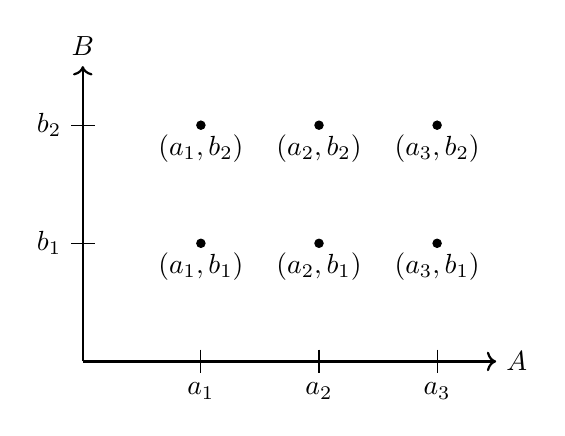
\begin{tikzpicture}[scale=1.5]
  % x軸とy軸
  \draw[->, thick] (0,0) -- (3.5,0) node[right] {$A$};
  \draw[->, thick] (0,0) -- (0,2.5) node[above] {$B$};  

  % ラベル(整数の目盛り)
  \foreach \x in {1, ...,3} {
    \draw (\x,0.1) -- (\x,-0.1) node[below] {$a_\x$};
  }
  \foreach \y in {1,...,2} {
    \draw (0.1,\y) -- (-0.1,\y) node[left] {$b_\y$};
  }
  \foreach \x in {1,...,3} {
    \foreach \y in {1,...,2} {
      \filldraw[black] (\x, \y) circle (1pt);
      \node[below] at (\x, \y) {$(a_{\x}, b_{\y})$};
    }
  }
\end{tikzpicture}
\end{center}
縦横の軸が直交している$XY$座標を「デカルト座標」ということを思い出せば,直積がなぜ「デカルト積」と呼ばれるのかの理由も腑に落ちるだろう.
実際,我々が慣れ親しんできた$XY$座標は,実数$\mathbb{R}$同士の直積$\mathbb{R} \times \mathbb{R}$である\footnote{もちろんこれは素材としての「集合」だけを考えれば,ということであって,本当はその上に位相などの構造が入る.}(これを$\mathbb{R}^2$と書くこともある).
同様に,$n$個の集合の積は,$n$次元空間の直交座標と類比的に考えることができる.


\begin{renshu}{}{}
$A \times B$ は $B \times A$と等しいだろうか.
\end{renshu}{}{} 

%
% 種は集合として定義できるだろうか


\section{ラッセルのパラドクス}
集合の内包的定義では,述語からその述語が該当する個物を集めた集合を作り出す.
ではどんな述語でも,対応した集合を作れるのだろうか?
ここで「自分自身を元として含まない」という述語を作り,これに対応する集合を$R$としよう.
つまり
\[
 R := \{x | x \text{は自分自身を元として含まない}\}.
\]
あるいは集合論的な記法をすれば
\[
 R := \{x | x \not \in x\}.
\]
こうして定義された$R$は様々な集合を元として持つ.
例えばビートルズのメンバーからなる集合$B$は,その内に$B$自身を含まない(「ビートルズ」というバンドの中に「ビートルズ」というメンバーはいない),つまり$B \not \in B$なので,$B \in R$である.
他にも,基本あらゆるものについて$R$の元かどうかを判断することができる(練習:$R$の元ではない集合にはどのようなものがあるか,考えてみよ).
では,$R$自身はどうだろうか?それは$R$に含まれるのか,そうではないのか.

実はどちらだと考えても,矛盾してしまう.まず,$R$は$R$に含まれない,と仮定してみよう.
\begin{itemize}
 \item[(a)] 仮定:$R \not\in R$.
 \item[(b)] するとこれは$R$の定義の条件を満たすので,$R$は$R$に含まれる,つまり$R \in R$.
 \item[(c)] これは仮定(a)と矛盾するので,背理法より(a)の反対,つまり$R \in R$が導かれる.
\end{itemize}
次に,$R$は$R$に含まれる,と仮定してみる.
\begin{itemize}
 \item[(a')] 仮定:$R \in R$.
 \item[(b')] するとこれは$R$の定義の条件を満たさないので,$R$は$R$に含まれない,つまり$R \not\in R$.
 \item[(c')] これは仮定(a')と矛盾するので,背理法より(a')の反対,つまり$R \not\in R$が導かれる.
\end{itemize}
つまり,$R \in R$かつ$R \not\in R$ということが導かれてしまう.
これはラッセルのパラドクス(Russell's paradox)として知られ,集合$R$はラッセル集合とよばれる.
バートランド・ラッセルは1902年にこのパラドクスの存在に気が付き,集合論的土台の上に数学を構築しようとしていたゴットロープ・フレーゲに書簡で知らせた.
当時,そのプロジェクトの集大成『算術の基本法則』をほぼ書き終えるところであったフレーゲは,自らの仕事の屋台骨に矛盾が含まれるというこの知らせに大変ショックを受けたという.

ラッセルのパラドクスは,内包的定義を無制限に適用すると矛盾を生んでしまう,ということを示している.
よってこれを回避するためには,「どんな述語にも対応する集合がある」ということをあきらめて,内法的定義に用いることができる述語に制約を加える必要がある.
現代の公理的集合論(例えばZFC集合論と呼ばれるものが一般的)は,何が集合として認められる(認められないか)をしっかりと公理で定めることで,ラッセル集合のような問題含みの「集合」が生じることを防いでいる(例えば,「すべての集合のあつまり」のようなものは集合としては認められない).



\bibliographystyle{apalike}
\bibliography{m4p}


\end{document}